%%%%%%%%%%%%%%%%%%%%%%%%%%%%%%%%%%%%%%%%%%%%%%%%%%%%%%%%%%%%%%%%%%%%%%%%%%%%%%%%
% AMS Beamer series / Bologna FC / Template
% Andrea Omicini
% Alma Mater Studiorum - Università di Bologna
% mailto:andrea.omicini@unibo.it
%%%%%%%%%%%%%%%%%%%%%%%%%%%%%%%%%%%%%%%%%%%%%%%%%%%%%%%%%%%%%%%%%%%%%%%%%%%%%%%%
%\documentclass[handout]{beamer}\mode<handout>{\usetheme{default}}
%
\documentclass[presentation]{beamer}\mode<presentation>{\usetheme{AMSBolognaFC}}
%\documentclass[handout]{beamer}\mode<handout>{\usetheme{AMSBolognaFC}}
%%%%%%%%%%%%%%%%%%%%%%%%%%%%%%%%%%%%%%%%%%%%%%%%%%%%%%%%%%%%%%%%%%%%%%%%%%%%%%%%
\usepackage{ske-ski-talk-2022}
% version
\newcommand{\versionmajor}{0}
\newcommand{\versionminor}{0}
\newcommand{\versionpatch}{1}
\newcommand{\version}{\versionmajor.\versionminor.\versionpatch}
%%%%%%%%%%%%%%%%%%%%%%%%%%%%%%%%%%%%%%%%%%%%%%%%%%%%%%%%%%%%%%%%%%%%%%%%%%%%%%%%
\title[Dive into \skeski]
{Dive into \longskeski}
%
\subtitle[gentle introduction and technologies]
{gentle introduction and technologies}
%

\author[\sspeaker{Magnini et al.} ]
{\speaker{Matteo Magnini}$^{*}$ \and Giovanni Ciatto$^{*}$}
%
\institute[DISI, Univ.\ Bologna]
{
    $^{*}$\disi\\\unibo
    \\
    \{\speaker{matteo.magnini}, giovanni.ciatto\}@unibo.it % emph the presenting author's email
}
%
\date[XAI project]{XAI project\\October 7, 2022, virtual}
%
\AtBeginSection[]
{
    %\\\\\\\\\\\\\\\\\\\\\
    \begin{frame}<beamer>[c,noframenumbering]
        \frametitle{Next in Line\ldots}
        \tableofcontents[sectionstyle=show/shaded,subsectionstyle=hide]
    \end{frame}
    %\\\\\\\\\\\\\\\\\\\\\
}
\AtBeginSubsection[]
{
    %\\\\\\\\\\\\\\\\\\\\\
    \begin{frame}<beamer>[shrink,noframenumbering]
        \frametitle{Focus on\ldots}
        \mbox{~}
        \tableofcontents[currentsubsection,sectionstyle=shaded,subsectionstyle=show/shaded]
        \mbox{~}
    \end{frame}
    %\\\\\\\\\\\\\\\\\\\\\
}
%
%%%%%%%%%%%%%%%%%%%%%%%%%%%%%%%%%%%%%%%%%%%%%%%%%%%%%%%%%%%%%%%%%%%%%%%%%%%%%%%%
\begin{document}
%%%%%%%%%%%%%%%%%%%%%%%%%%%%%%%%%%%%%%%%%%%%%%%%%%%%%%%%%%%%%%%%%%%%%%%%%%%%%%%%

%/////////
\frame{\titlepage}
%/////////

%%===============================================================================
%\section*{Outline}
%%===============================================================================
%
%%/////////
%\frame[c]{\tableofcontents[hideallsubsections]}
%%/////////


%===============================================================================
\section{Premises}
%===============================================================================

\begin{frame}[c]{Presentation}
    
    \begin{block}{Not only myself}
        \begin{itemize}
            \item \emph{Andrea Agiollo}, \unibo{} \disi{};
            %
            \item \emph{Andrea Omicini}, \unibo{} \disi{};
            %
            \item \emph{Andrea Rafanelli}, \unipi{} \di{}, \uniaq{} \disim{};
            %
            \item \emph{Federico Sabbatini}, \uniurb{} \dispea{};
            %
            \item \emph{Giovanni Ciatto}, \unibo{} \disi{};
            %
            \item \emph{Matteo Magnini}, \unibo{} \disi{};
        \end{itemize}
    \end{block}

\end{frame}

\begin{frame}[c]{Concerning human (and machine) reasoning}
    
    \begin{block}{The three ways}
        \begin{itemize}
            \item \alert{induction}\\
            %
            a kind of reasoning that uses particular examples in order to reach a general conclusion about something\\
            %
            $\rightarrow$ machine learning (e.g., neural networks);
            %
            \item \alert{deduction}\\
            %
            the act or process of using logic or reason to form a conclusion or opinion about something\\
            %
            $\rightarrow$ symbolic artificial intelligence (e.g., logic programs);
            %
            \item \alert{abduction}\\
            %
            the forming and accepting on probation of a hypothesis to explain surprising facts\\
            %
            $\rightarrow$ abductive logic programming.
        \end{itemize}
    \end{block}

\end{frame}


\begin{frame}[allowframebreaks]{Concepts we need to know}

    %
    \begin{block}{Symbolic knowledge}
        A symbolic representation of knowledge consists of: \ccite{sub-symbolic-vs-symbolic}
        %
        \begin{enumerate}
            \item a set of symbols;
            \item\label{item:symbolic-combination} a set of grammatical rules governing the combining of symbols; 
            \item\label{item:symbolic-assignment} elementary symbols and any admissible combination of them can be assigned with meaning.
            %
            \begin{itemize}
                \item[$\Rightarrow$] Symbolic knowledge is both human and machine interpretable,
                \item first order logic (FOL) is an example of symbolic representation.
            \end{itemize}
        \end{enumerate}
    \end{block}
    
    \framebreak

    %/////////
    \begin{block}{Sub-symbolic data}
    \begin{itemize}
        \item ML methods, and sub-symbolic approaches in general, represent data as arrays of real numbers, and knowledge as functions over such data;
        %
        \item despite numbers are technically symbols as well, we cannot consider arrays and their functions as symbolic knowledge representation (KR) means;
        %
        \item sub-symbolic approaches frequently violate \Cref{item:symbolic-combination,item:symbolic-assignment}.
        %
    \end{itemize}
    %
    \end{block}
    %/////////
    
    \framebreak
    
    %
    \begin{block}{Local representation}
        \begin{itemize}
            \item Each number of the array has a well-defined meaning;
            %
            \item example $\rightarrow$ iris dataset sample, array with 5 elements where each element has meaning (sepal/petal length/width and class).
        \end{itemize}    
    \end{block}

    \begin{block}{Distributed representation}
        \begin{itemize}
            \item Each number of the array is meaningless, unless it is considered along with its neighbourhood;
            %
            \item example $\rightarrow$ images represented as $w\ x\ h$ matrices of numbers in range $[0,1]$.
            %
            (Violation of \cref{item:symbolic-assignment})
        \end{itemize}
    \end{block}
    
    \framebreak
    
     \begin{figure}
        \centering
        \subfloat{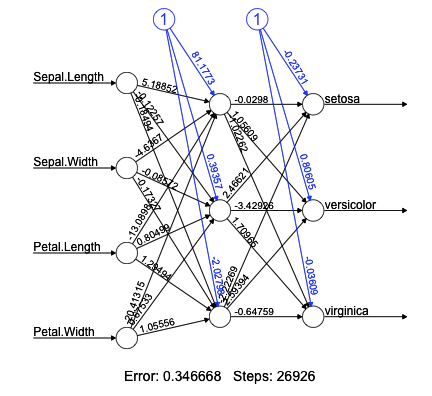
\includegraphics[width=0.4\textwidth]{figures/nn-iris}}
        %
        \qquad
        %
        \centering
        \subfloat{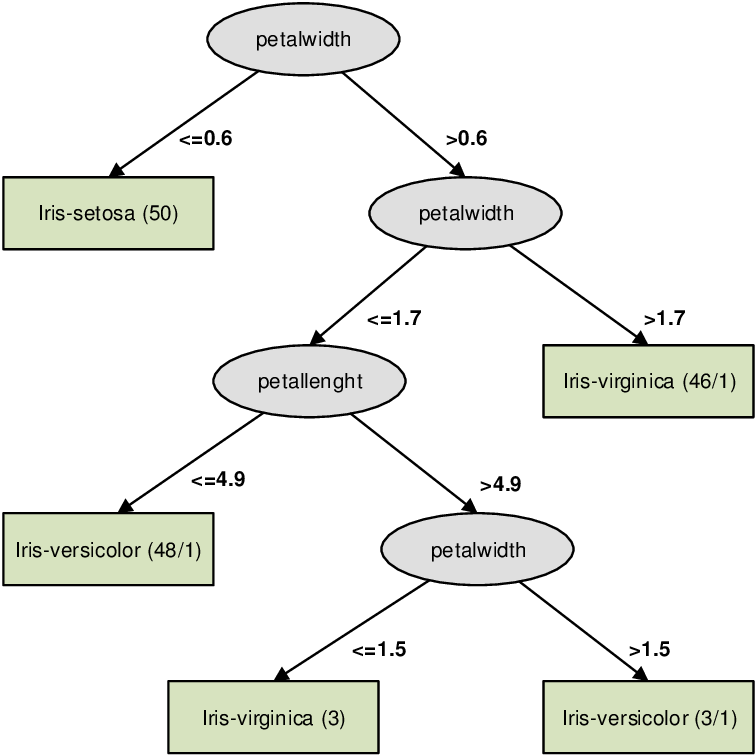
\includegraphics[width=0.4\textwidth]{figures/decision-tree-iris}}
    \end{figure}
    
    \framebreak
    
    Set of propositional logic rules built from the previous decision tree:
    
    \begin{equation*}
        \begin{aligned}
            \pred{iris}&(\var{SepalLenght}, \var{SepalWidth}, \var{PetalLenght}, \var{PetalWidth}, \const{setosa})\text{:-}\\
            &\var{PetalWidth} =< 0.6.\\
            \pred{iris}&(\var{SepalLenght}, \var{SepalWidth}, \var{PetalLenght}, \var{PetalWidth}, \const{versicolor}) \text{:-}\\
            &\var{PetalWidth} > 0.6, \var{PetalWidth} =< 1.7, \var{PetalLenght} =< 4.9.\\
            \pred{iris}&(\var{SepalLenght}, \var{SepalWidth}, \var{PetalLenght}, \var{PetalWidth}, \const{virginica}) \text{:-}\\
            &\var{PetalWidth} > 0.6, \var{PetalWidth} =< 1.5, \var{PetalLenght} > 4.9.\\
            \pred{iris}&(\var{SepalLenght}, \var{SepalWidth}, \var{PetalLenght}, \var{PetalWidth}, \const{versicolor}) \text{:-}\\
            &\var{PetalWidth} > 1.5, \var{PetalWidth} =< 1.7, \var{PetalLenght} > 4.9.\\
            \pred{iris}&(\var{SepalLenght}, \var{SepalWidth}, \var{PetalLenght}, \var{PetalWidth}, \const{virginica}) \text{:-}\\
            &\var{PetalWidth} > 1.7.\\
        \end{aligned}
    \end{equation*}
    
    \framebreak
    
    Interpretability vs performance trade-off
    \centering
    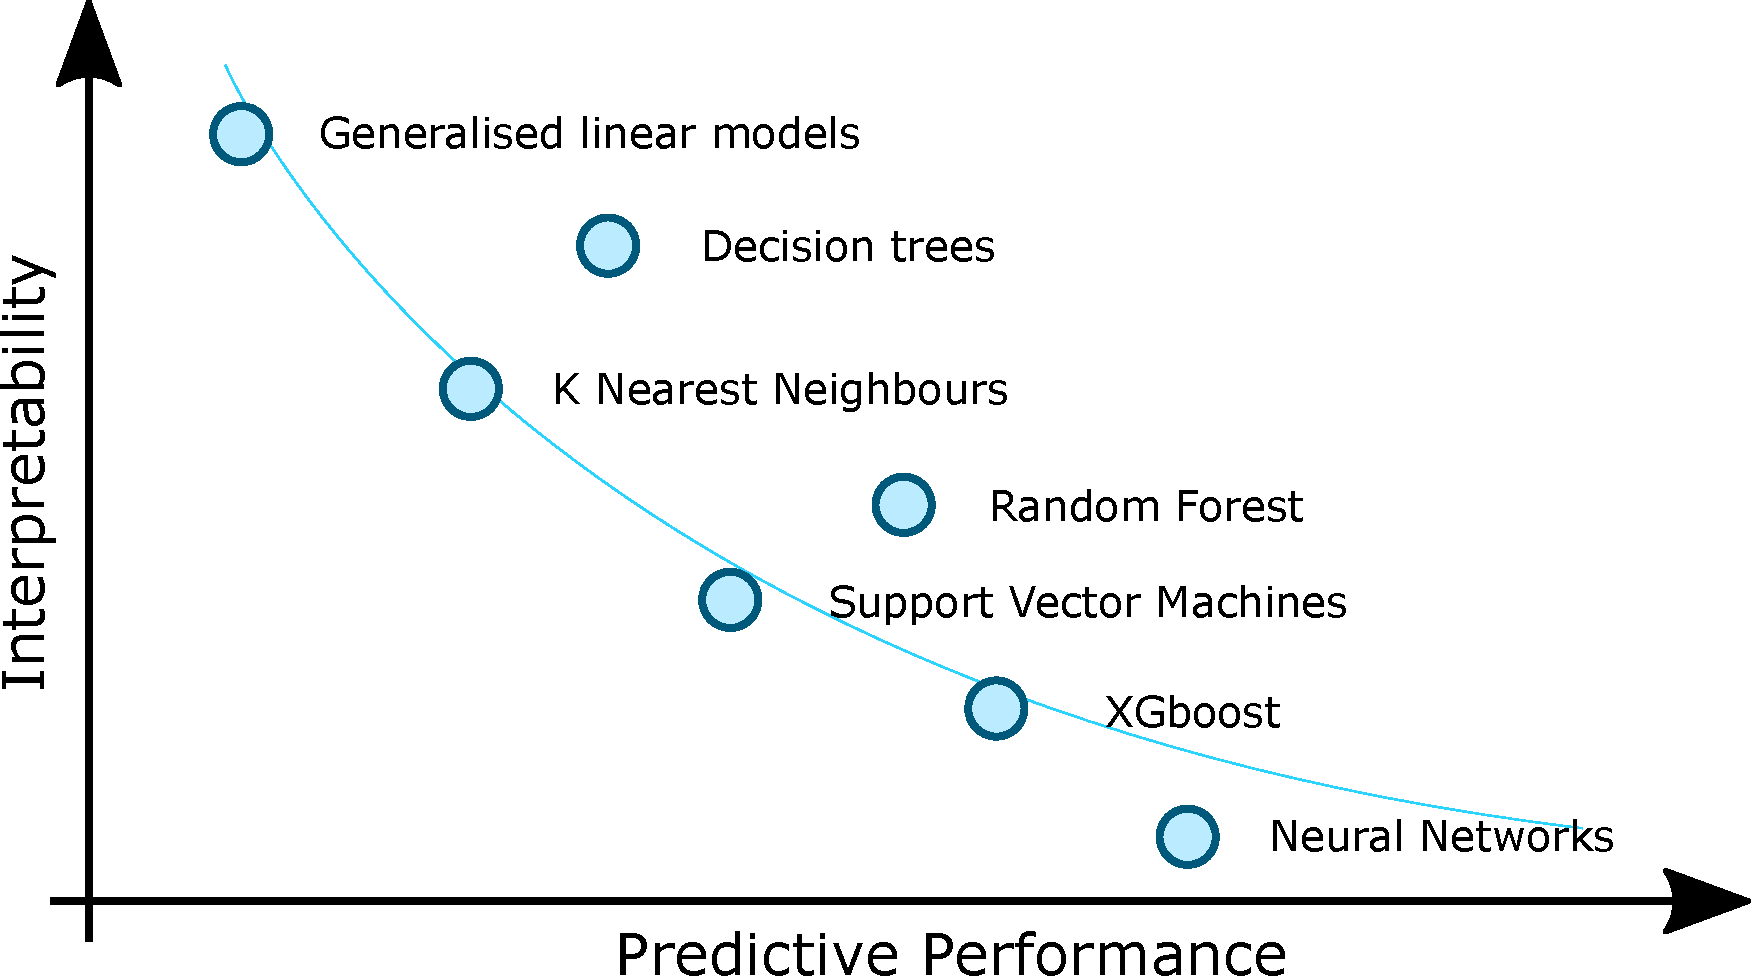
\includegraphics[width=0.8\textwidth]{figures/interpretability-performance-tradeoff}
    
\end{frame}
%/////////


%===============================================================================
\section{\longske}
%===============================================================================


%/////////
\begin{frame}[c]{Definition}
    \begin{block}{We define \longske{} (\ske) as: \ccite{andrews1995survey,GarcezBG01,Hailesilassie16,ZilkeMJ16,guidotti2018survey}}
        \begin{displayquote}\itshape
            any \emph{algorithmic} procedure accepting \emph{trained} \alert{sub-symbolic predictors} as input and producing \alert{symbolic knowledge} as output, in such a way that the extracted knowledge \emph{reflects} the behaviour of the predictor with high fidelity.
        \end{displayquote}
        %
    \end{block}
    %
    \begin{block}{Notes}
        \begin{itemize}
            \item This will be just a brief introduction, I will focus more on \longski{} rather than \longske;
            %
            \item for more details and questions about \ske{} please contact\\$\rightarrow$ \emph{Federico Sabbatini} \href{mailto:f.sabbatini@unibo.it}{f.sabbatini@unibo.it}
        \end{itemize}
    \end{block}
    
\end{frame}
%/////////


%/////////
\begin{frame}[c]{Why \ske?}
    
    Explainability \ccite{darpa2016-xai} can be achieved:
    %
    \begin{block}{By post-hoc explanation}
        \begin{itemize}
            \item applying an algorithm of symbolic knowledge extraction on a trained predictor;
            %
            \item output $\rightarrow$ logic rules (or other symbolic means) that describe the predictor's behaviour.
            %
        \end{itemize}    
    \end{block}
    
\end{frame}
%/////////

\begin{frame}[allowframebreaks]{Taxonomy}
    \begin{block}{Translucency}
       What kind of ML predictor does the \ske{} method support?
        %
        \begin{itemize}
            \item pedagogical: any supervised predictor
            \item decompositional: a particular sort of ML predictor (e.g., NN, SVM, DT)      
        \end{itemize} 
     \end{block}

    \begin{block}{Input data}
        \begin{itemize}
            \item binary: $\mathcal{X} \equiv \{0, 1\}^n$
            \item discrete: $\mathcal{X} \in \{x_1, \ldots, x_n\}^n$   
            \item continuous: $\mathcal{X} \subseteq \mathbb{R}^n$     
        \end{itemize} 
    \end{block}
        
    \framebreak
        
    \begin{block}{Output shape}
        \begin{itemize}
            \item rule list: i.e. ordered sequences of if-then-else rules
            \item decision tree: hierarchical set of if-then-else rules involving a comparison among a variable and a constant   
            \item decision table: 2D tables summarising decisions for each possible assignment of variables 
        \end{itemize} 
    \end{block}
        
    \framebreak
        
    \begin{block}{Output expressiveness}
        %
        \begin{itemize}
            \item propositional: boolean statements + logic connectives
            %
            \begin{itemize}
                \item there including arithmetic comparisons among variables and constants
            \end{itemize}
            
            \item fuzzy: hierarchical set of if-then-else rules involving a comparison among a variable and a constant   
            \item oblique: boolean statements + logic connectives + arithmetic comparisons
            \item M-of-N: any of the above + statements like $m-\text{of}-\{\phi_1, \ldots, \phi_n \}$
        \end{itemize} 
        
    \end{block}
\end{frame}


%===============================================================================
\section{\longpsyke}
%===============================================================================

\begin{frame}[c]{Gentle presentation}
    \begin{block}{\longpsyke{} (\psyke) \ccite{psyke-woa2021}}
        \begin{itemize}
            \item \psyki is intended as a library of \ske{} algorithms for data/computer scientists;
            %
            \item it is written in Python and it is compliant with scikit-learn standard nomenclature, i.e., you can call a \ske{} algorithm upon a Ml model that has the \texttt{predict} method;
            %
            \item code is public available on \href{https://github.com/psykei/psyke-python}{https://github.com/psykei/psyke-python}
            %
            \item to install run \texttt{pip install psyke}
            %
            \item currently \psyke{} supports several \ski{} algorithms, among which:
            \begin{itemize}
                \item \longcart{} (\cart) \ccite{cart1984}
                \item \longreal{} (\real) \ccite{real1994}
                \item \trepan{} \ccite{trepan1996}
                \item \iter{} \ccite{iter2006}
                \item \gridex{} \ccite{gridex-extraamas2021}
            \end{itemize}
        \end{itemize}
    \end{block}
\end{frame}


%===============================================================================
\section{\longski}
%===============================================================================
    
%/////////
\begin{frame}[c]{Definition}
    \begin{block}{We define \longski{}(\ski) as: \ccite{surveyNeuroSymb,surveyXie,surveyCalegariCO20}}
        \begin{displayquote}\itshape
            any \emph{algorithmic} procedure affecting how \alert{sub-symbolic predictors} draw their inferences in such a way that predictions are either \emph{computed} as a function of, or made \emph{consistent} with, some \emph{given} \alert{symbolic knowledge}.
        \end{displayquote}
    \end{block}
    
\end{frame}
%/////////


%/////////
\begin{frame}[allowframebreaks]{Why \ski?}
    \begin{block}{There are several benefits:}
        %
        \begin{itemize}
            %
            \item prevent the predictor to become a black-box\alert{!};
            %
            \item reduce learning time;
            %
            \item reduce the data size needed for training;
            %
            \item improve predictor's accuracy;
            %
            \item build a predictor that behave as a logic engine.
        \end{itemize}
        %
    \end{block}

     \framebreak

    Explainability \ccite{darpa2016-xai} can be achieved:
    
    \begin{block}{By design}
        \begin{itemize}
            \item constraining the behaviour of predictors that are natively black-boxes with symbolic knowledge;
            %
            \item structuring the predictor's architecture with symbolic knowledge;
            %
            \item output $\rightarrow$ a predictor that does not violate the prior knowledge.
        \end{itemize}
    \end{block}
    
\end{frame}
%/////////

\begin{frame}[c]{Taxonomy}
    \begin{block}{Dimensions}
        \begin{itemize}
            \item Aim $\rightarrow$ main purpose of the injection;
            \item Predictors $\rightarrow$ target of the injection;
            \item How $\rightarrow$ in which way the injection is performed;
            \item Logic $\rightarrow$ what kind of logic formalism is used to represent knowledge.
        \end{itemize}
    \end{block}
\end{frame}
    
\begin{frame}[c]{Aim}
    \begin{block}{Enrich (learning support)}
        \begin{itemize}
            \item reduce learning time;
            %
            \item reduce the data size needed for training;
            %
            \item improve predictor's accuracy.
        \end{itemize}
    \end{block}
    %
    \begin{block}{Manifold (symbolic knowledge manipulation)}
    \begin{itemize}
        \item logic inference;
        %
        \item information retrieval;
        %
        \item knowledge base completion/fusion.
    \end{itemize}
    \end{block}
\end{frame}
%/////////

\begin{frame}[c]{Predictors}
    \begin{block}{What kind of predictors are feasable for \ski?}
        \begin{itemize}
            \item in theory every sub-symbolic predictors;
            %
            \item in particular (deep) neural networks are the preferred targets for several reasons:
            %
            \begin{itemize}
                \item easy to manipulate;
                %
                \item high performance;
                %
                \item technological maturity.
            \end{itemize}
        \end{itemize}
    \end{block}
\end{frame}
%/////////


%/////////
\begin{frame}[allowframebreaks]{How}
    \begin{block}{Injection families}
        %
        There exist three major ways to perform knowledge injection on sub-symbolic predictors:
        %
        \begin{itemize}
            \item \alert{constraining}, a cost factor proportional to the violation of the knowledge is introduced during learning;
            \item \alert{structuring}, the architecture of the predictor is built in such a way to mimic the knowledge;
            \item \alert{embedding}, the symbolic knowledge is embedded into a tensor form and it is given in input as training data to the predictor.
        \end{itemize} 
    \end{block}
    %
    
    \framebreak

    \begin{block}{Constraining}
       \begin{itemize}
           \item Knowledge cost factor is introduced in the loss function;
           %
           \item for NN the cost affects backpropagation \ccite{backpropagation} during training.
           %
           \begin{itemize}
               \item[$\Rightarrow$] Predictor does not violate the prior knowledge (to a certain extent).
           \end{itemize} 
       \end{itemize}
       
       \begin{figure}
           \centering
           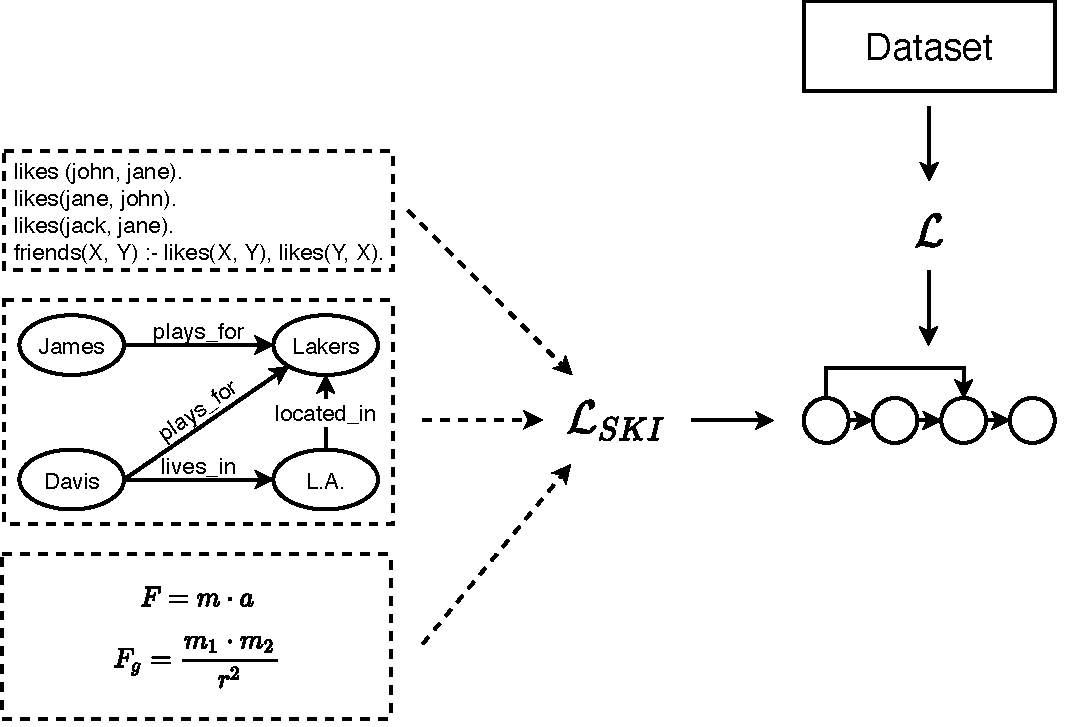
\includegraphics[width=0.4\textwidth]{figures/ski-constraining}
       \end{figure}
       %
    \end{block}
    
    \framebreak
    
    \begin{block}{Structuring}
         \begin{itemize}
            \item Inner architecture is shaped to be able to ``mimic'' the knowledge;
            %
            \item for NN this means \emph{ad-hoc} layers.
            %
            \begin{itemize}
                \item[$\Rightarrow$] Predictor directly exploits knowledge when needed.
            \end{itemize} 
        \end{itemize}
        %
        \begin{figure}
            \centering
            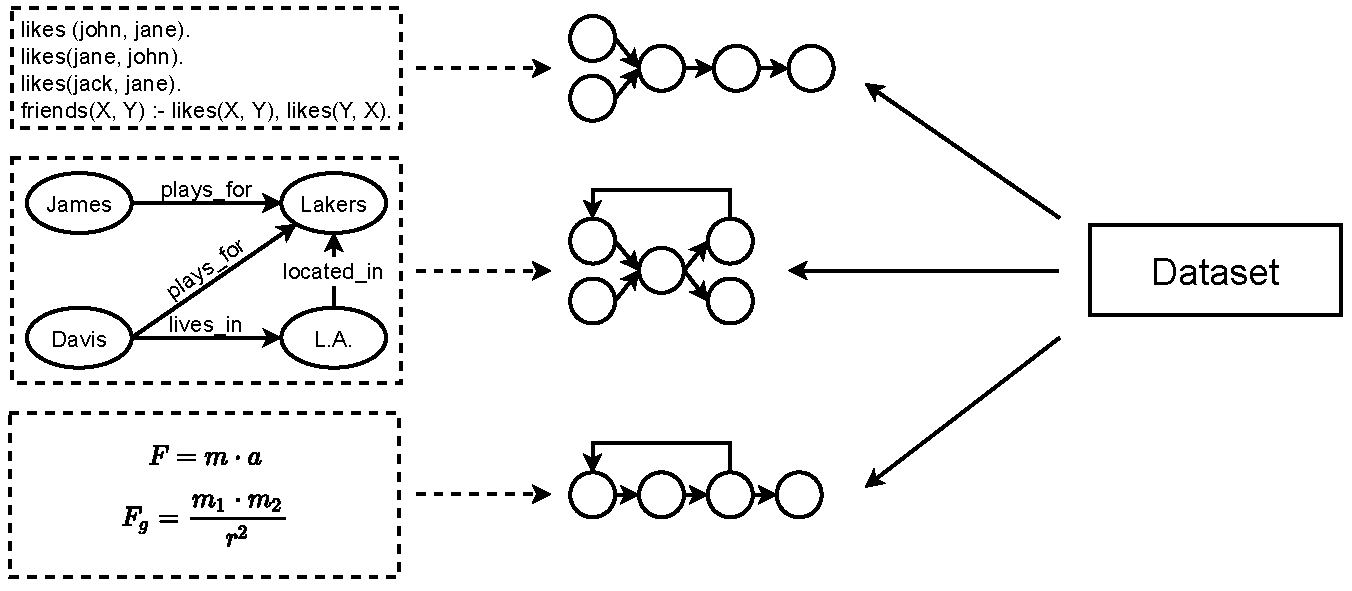
\includegraphics[width=0.6\textwidth]{figures/ski-structuring}
        \end{figure}
        %
    \end{block}

    \framebreak
   
    %
    \begin{block}{Embedding}
        \begin{itemize}
            \item Symbolic knowledge is embedded into a tensor form;
            %
            \item this is used as predictor's input data (alone or with a ``standard'' dataset).
            %
            \begin{itemize}
                \item[$\Rightarrow$] Predictor's aim is manifold in most cases.
            \end{itemize} 
        \end{itemize}
        
        \begin{figure}
            \centering
            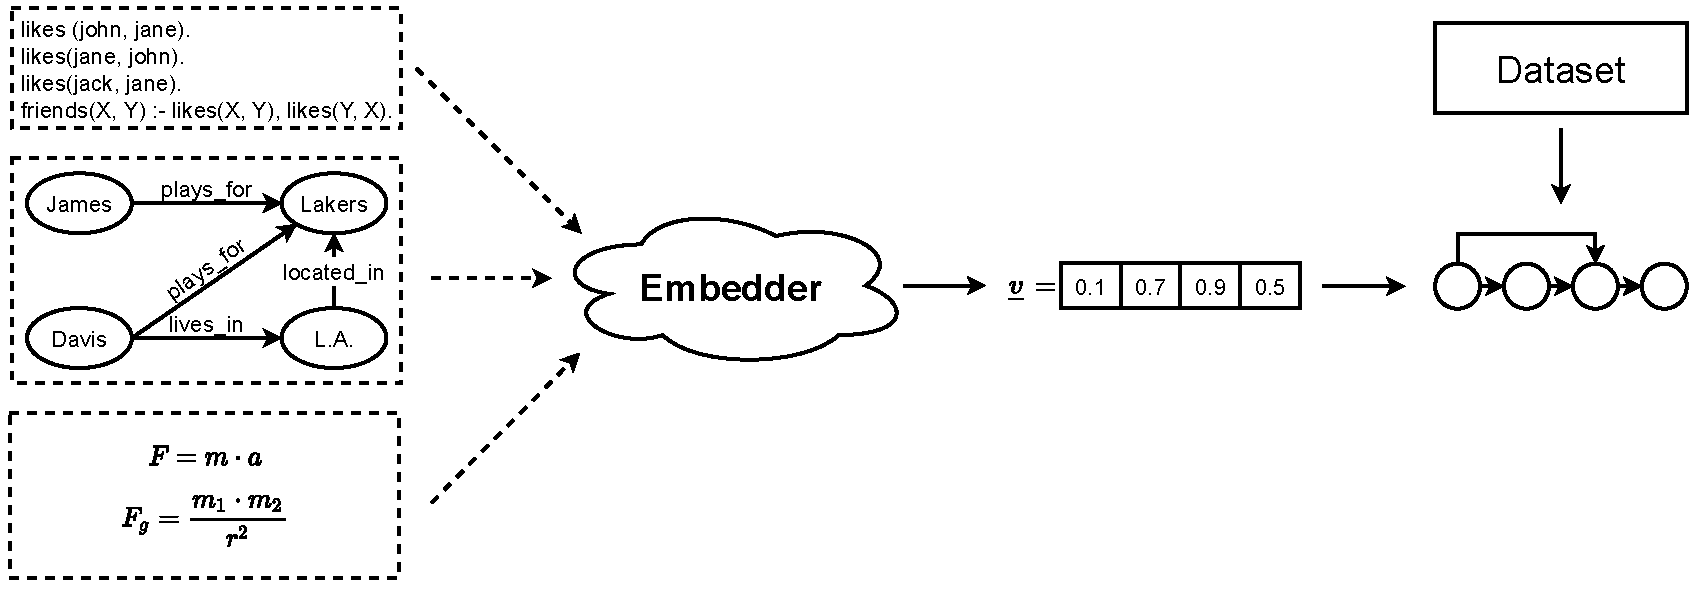
\includegraphics[width=0.6\textwidth]{figures/ski-embedding}
        \end{figure}
    \end{block}
\end{frame}
%/////////


\begin{frame}[allowframebreaks]{Logic}
    \begin{block}{Intensional}
        \begin{itemize}
            \item indirect representation of data,
            %
            \item define a relation/set by describing its elements via other relations/sets.
        \end{itemize}
        %
    \end{block}
    %
    \begin{block}{Extensional}
        \begin{itemize}
            \item direct representation of data,
            %
            \item explicit definition of entities involved.
        \end{itemize}
    \end{block}
    
    \framebreak
    
    \begin{block}{Most used logic formalisms}
        \begin{itemize}
            \item Recursive intensional predicates are very expressive and powerful, as they enable the description of infinite sets via a finite (and commonly small) amount of formul\ae;
            \item however, most sub-symbolic predictors are NN, the vast majority of them are direct acyclic graph (DAG) $\rightarrow$ no support to recursion;
            \item therefore one of the most common logic is just \alert{propositional logic (PL)} followed by \alert{knowledge graph (KG)} and then by \alert{first order logic (FOL)}.
        \end{itemize}
    \end{block}
\end{frame}



%===============================================================================
\section{\longpsyki}
%===============================================================================


\begin{frame}[allowframebreaks]{Gentle presentation}
    \begin{block}{\longpsyki{} (\psyki) \ccite{psyki-extraamas2022}}
        \begin{itemize}
            \item \psyki is intended as a library of \ski{} algorithms for data/computer scientists;
            %
            \item it is written in Python and supports Tensorflow;
            %
            \item code is public available on \href{https://github.com/psykei/psyki-python}{https://github.com/psykei/psyki-python}
            %
            \item to install run \texttt{pip install psyki}
            %
            \item currently \psyki{} supports the following \ski{} algorithms:
            \begin{itemize}
                \item \longkins{} (\kins) \ccite{kins-cilc2022}
                \item \longkill{} (\shortkill) \ccite{kill-woa2022}
                \item \longkbann{} (\kbann) \ccite{KBANN-origin}
            \end{itemize}
        \end{itemize}
    \end{block}

    \framebreak
    
    General code snippet for \psyki{} usage.
    \lstinputlisting[
    language=Python,
    basicstyle=\ttfamily\tiny,
    label=lst:code,
    captionpos=b,
    ]{listings/kins-snippet.py}
    
\end{frame}



%/////////
\begin{frame}[allowframebreaks]{Knowledge Injection via Network Structuring}
    
    \begin{block}{KINS: Knowledge Injection via Network Structuring}
        %
        A general SKI algorithm that does not impose constrains on the sub-symbolic predictor to enrich.
        %
        \begin{itemize}
            %
            \item aim $\rightarrow$ enrich;
            %
            \item predictor $\rightarrow$ neural network;
            %
            \item how $\rightarrow$ structuring;
            %
            \item logic $\rightarrow$ stratified Datalog with negation.
            %    
        \end{itemize}        
    \end{block}
    
    \framebreak
    
    \begin{figure}
        \centering
        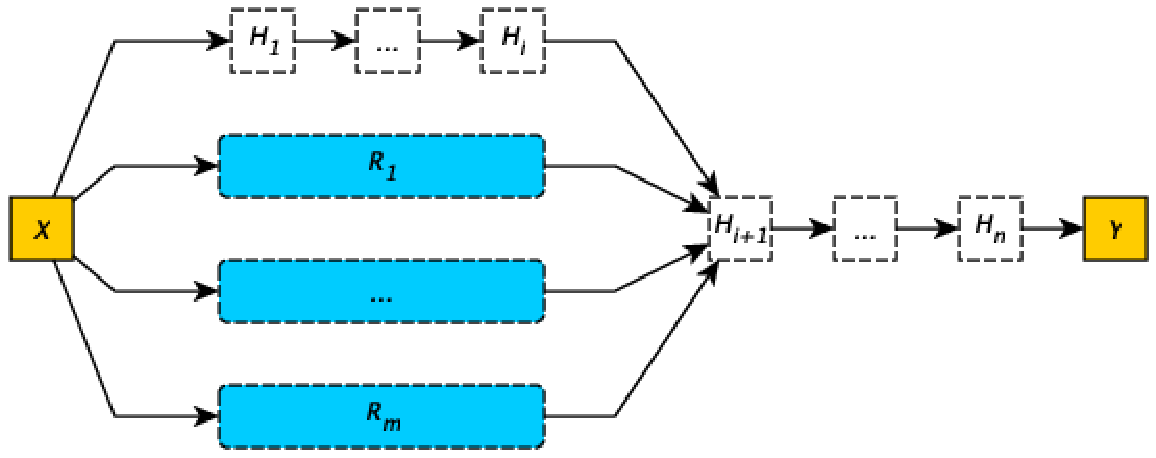
\includegraphics[width=0.8\textwidth]{figures/kins-architecture}
    \end{figure}
    
    \framebreak
    
    \resizebox{\textwidth}{!}{
    \begin{tabular}{l|r||l|r}
        \textbf{Formula} & \textbf{C. interpretation} & \textbf{Formula} & \textbf{C. interpretation}
        \\
        \hline\hline
        $\llbracket\neg \phi\rrbracket$ & $\eta\{1 - \llbracket\phi\rrbracket\}$ & $\llbracket\phi \leftarrow \psi\rrbracket$ & $\eta\{min\{1, 1-\llbracket\phi\rrbracket+\llbracket\psi\rrbracket\}\}$ % Negation % Left Implication
        \\
        $\llbracket\phi  \wedge \psi\rrbracket$ &  $\eta\{min\{\llbracket\phi\rrbracket, \llbracket\psi\rrbracket\}\}$ & $\llbracket\phi \leftrightarrow \psi\rrbracket$ & $\eta\{min\{1, 1-|\llbracket\phi\rrbracket-\llbracket\psi\rrbracket|\}\}$ % Conjunction % Double Implication
        \\
        $\llbracket\phi  \vee \psi\rrbracket$ & $\eta\{max\{\llbracket\phi\rrbracket, \llbracket\psi\rrbracket\}\}$ & $\llbracket \text{expr}(\bar{X}) \rrbracket$ & $\text{expr}(\llbracket\bar{X}\rrbracket)$ % Disjunction
        \\
        $\llbracket\phi = \psi\rrbracket$ & $\eta\{\llbracket\neg( \phi \ne \psi )\rrbracket \}$ &$\llbracket \mathtt{true} \rrbracket$ & $1$ % Equal
        \\
        $\llbracket\phi \ne \psi\rrbracket$ & $\eta\{|\llbracket\phi\rrbracket-\llbracket\psi\rrbracket|\}$ & $\llbracket \mathtt{false} \rrbracket$ & $0$ % Not Equal
        \\
        $\llbracket\phi > \psi\rrbracket$ & $\eta\{max\{0, \llbracket\phi\rrbracket - \llbracket\psi\rrbracket\}\}$ & $\llbracket X \rrbracket$ & $x$ % Greater
        \\
        $\llbracket\phi \ge \psi\rrbracket$  & $\eta\{\llbracket( \phi > \psi ) \vee ( \phi = \psi )\rrbracket\}$ & $\llbracket \const{k} \rrbracket$ & $k$ % Greater Equal
        \\
        $\llbracket\phi < \psi\rrbracket$  &  $\eta\{max\{0, \llbracket\psi\rrbracket - \llbracket\phi\rrbracket\}\}$ & $\llbracket \pred{p}(\bar{X}) \rrbracket^{**}$ & $\llbracket \psi_1 \vee \ldots \vee \psi_k \rrbracket$ % Less
        \\
        $\llbracket\phi \le \psi\rrbracket$  & $\eta\{\llbracket( \phi < \psi ) \vee ( \phi = \psi )\rrbracket\}$ & $\llbracket \pred{class}(\bar{X}, \const{y}_i) \leftarrow \psi \rrbracket$ & $\llbracket \psi \rrbracket^{*}$ % Less Equal
        \\
        $\llbracket\phi \rightarrow \psi\rrbracket$ & $\eta\{min\{1, 1- \llbracket\psi\rrbracket+\llbracket\phi\rrbracket\}\}$ & & % Right Implication        
    \end{tabular}
}
\begin{center}\scriptsize
    $^{*}$ encodes the value for the $i^{th}$ output
    \\
    \smallskip
    $^{**}$ assuming $p$ is defined by $k$ clauses of the form:
    \\
    $\pred{p}(\bar{X}) \leftarrow \psi_1,\ \ldots,\ \pred{p}(\bar{X}) \leftarrow \psi_k$
\end{center}
    
    \framebreak
    
    \begin{figure}
        \centering
        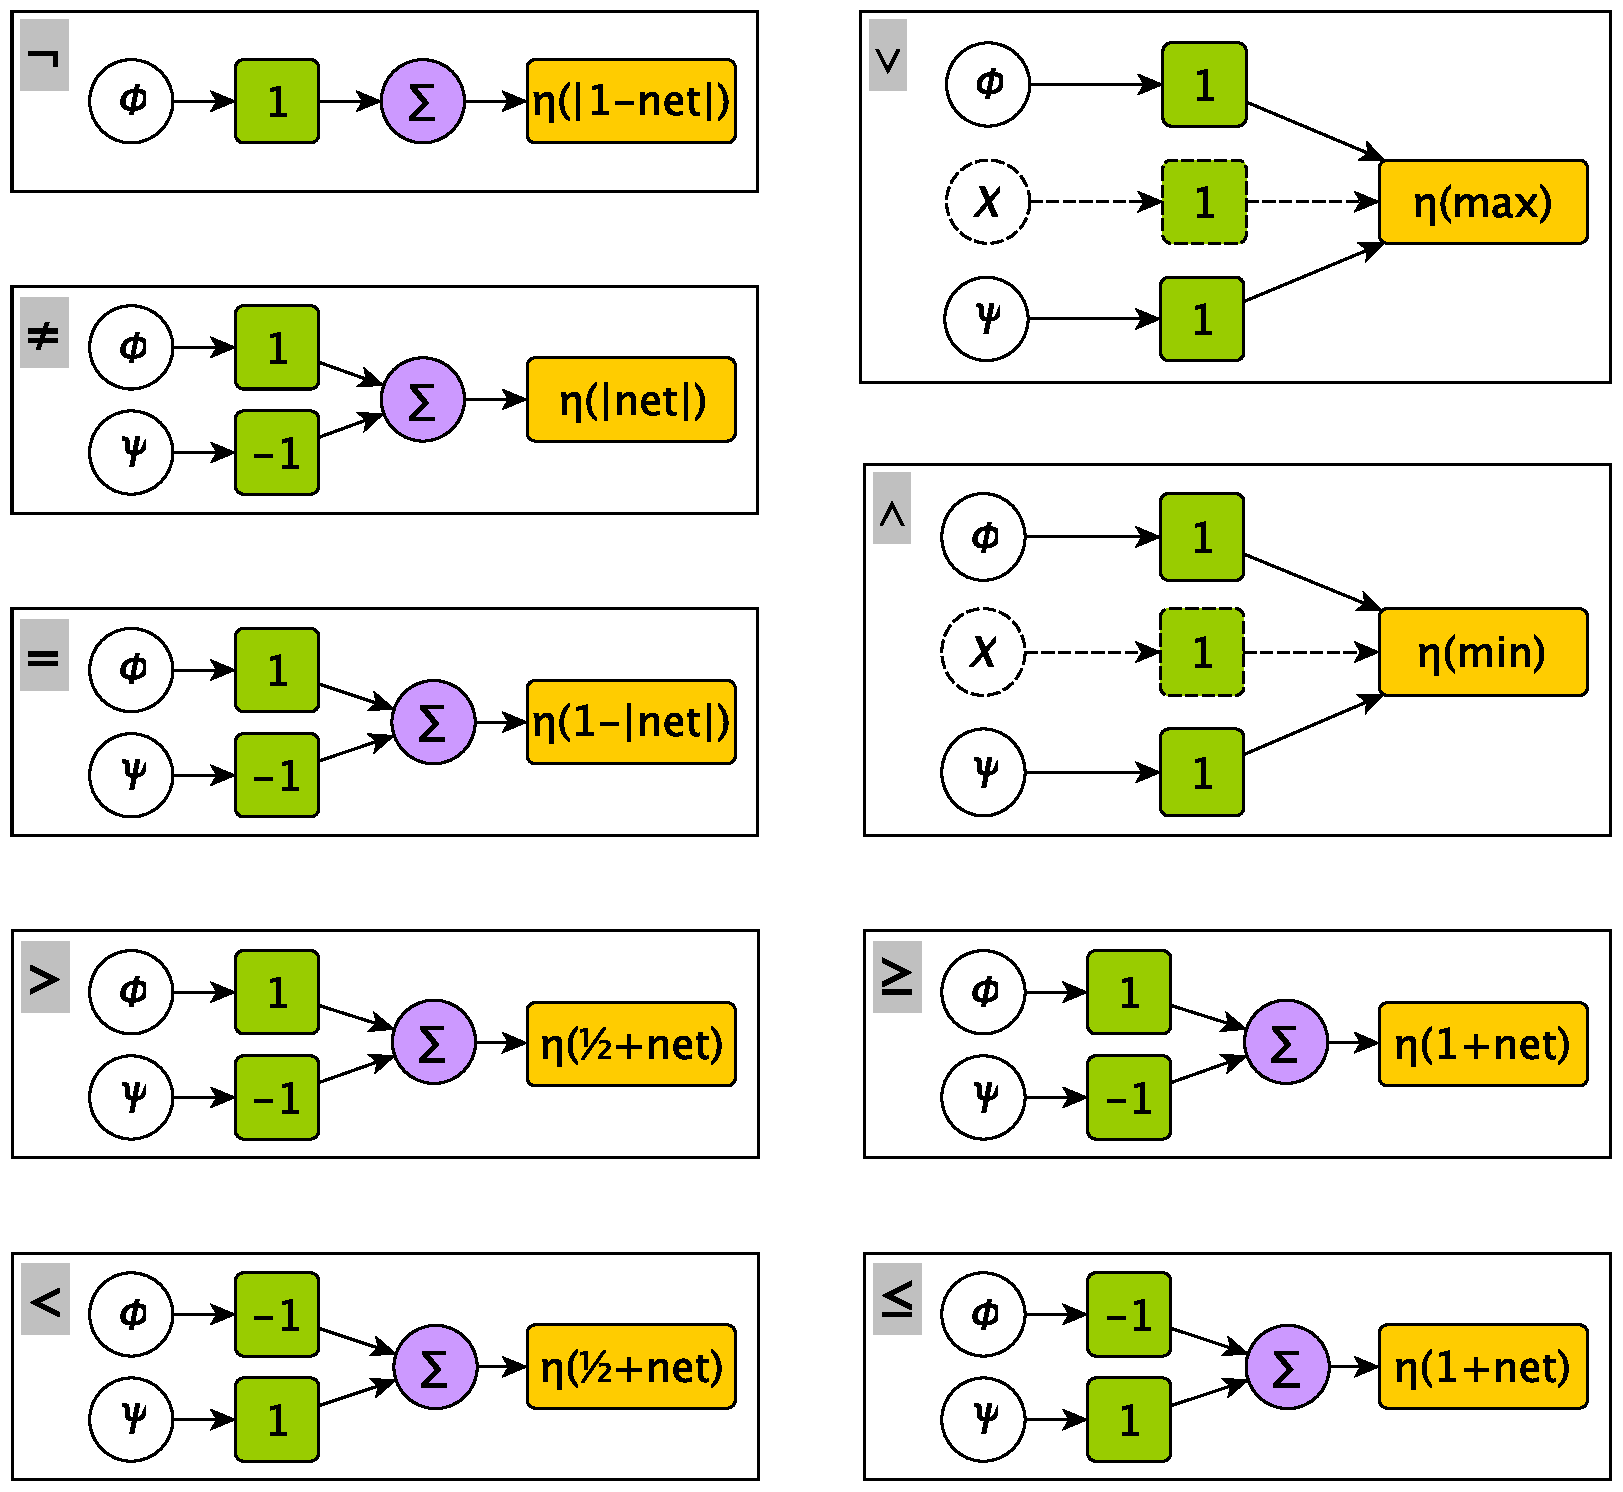
\includegraphics[width=0.65\textwidth]{figures/neurons}
    \end{figure}
    
\end{frame}
%/////////

%/////////
\begin{frame}[fragile,allowframebreaks]{Case study}
    %
    PSJGS: \href{https://archive.ics.uci.edu/ml/datasets/Molecular+Biology+(Splice-junction+Gene+Sequences)}{Primate Splice-Junction Gene Sequences dataset}
    %
    \begin{minipage}{0.5\textwidth}
        \begin{lstlisting}[language={}, basicstyle=\ttfamily\tiny,frame=none]
        EI-stop ::- @-3 'TAA'.
        EI-stop ::- @-3 'TAG'.
        EI-stop ::- @-3 'TGA'.
        EI-stop ::- @-4 'TAA'.
        EI-stop ::- @-4 'TAG'.
        EI-stop ::- @-4 'TGA'.
        EI-stop ::- @-5 'TAA'.
        EI-stop ::- @-5 'TAG'.
        EI-stop ::- @-5 'TGA'.
        
        IE-stop ::- @1 'TAA'.
        IE-stop ::- @1 'TAG'.
        IE-stop ::- @1 'TGA'.
        IE-stop ::- @2 'TAA'.
        IE-stop ::- @2 'TAG'.
        IE-stop ::- @2 'TGA'.
        IE-stop ::- @3 'TAA'.
        IE-stop ::- @3 'TAG'.
        IE-stop ::- @3 'TGA'.
        
        pyramidine-rich :- 6 of (@-15 'YYYYYYYYYY').
        
        EI :- @-3 'MAGGTRAGT', not(EI-stop).
        
        IE :- pyramidine-rich, @-3 'YAGG', not(IE-stop).
        \end{lstlisting}
    \end{minipage}
    \vline
    \begin{minipage}{0.45\textwidth}
        \begin{lstlisting}[language={}, basicstyle=\ttfamily\tiny,frame=none]           
    Class, Id, DNA-sequence
    
    EI,ATRINS-DONOR-521,CCAGCTGCAT...AGCCAGTCTG
    EI,ATRINS-DONOR-905,AGACCCGCCG...GTGCCCCCGC
    EI,BABAPOE-DONOR-30,GAGGTGAAGG...CACGGGGATG
    ...
    IE,ATRINS-ACCEPTOR-701,TTCAGCGGCC...GCCCTGTGGA
    IE,ATRINS-ACCEPTOR-1678,GGACCTGCTC...GGGGGCTCTA
    IE,BABAPOE-ACCEPTOR-801,GCGGTTGATT...AAGATGAAGG
    ...
    N,AGMKPNRSB-NEG-1,CAAAAGAACA...CAAGGCTACA
    N,AGMORS12A-NEG-181,AGGGAGGTGT...GGGCATGGGG
    N,AGMORS9A-NEG-481,TGGTCAATTC...TCTTGCTCTG
    ...
    
    3190 Records
        \end{lstlisting}
    \end{minipage}
    
    \framebreak
    
    \centering
\resizebox*{!}{0.8\textheight}{
    \centering
    \begin{adjustbox}{width=\linewidth, center}
        \centering
        \begin{tabular}{c|l}
            \centering
            \textbf{Class} & \textbf{Logic Formulation}
            \\\hline\hline
            \emph{EI} & $\begin{array}{l}
                \begin{aligned}
                    \pred{class}(\bar{\var{X}}, \const{ei}) \leftarrow& \var{X}_{-3} = \const{m} \wedge \var{X}_{-2} = \const{a} \wedge \var{X}_{-1} = \const{g} \wedge \var{X}_{+1} = \const{g}\ \wedge\\
                    & \var{X}_{+2} = \const{t} \wedge \var{X}_{+3} = \const{a} = \const{r} \wedge \var{X}_{+4} = \const{a}\ \wedge \\
                    & \var{X}_{+5} = \const{g} \wedge \var{X}_{+6} = \const{t} \wedge \neg(\pred{ei\_stop}(\bar{\var{X}}))
                \end{aligned}
                \\
                \pred{ei\_stop}(\bar{\var{X}}) \leftarrow \var{X}_{-3} = \const{t} \wedge \var{X}_{-2} = \const{a} \wedge \var{X}_{-1} = \const{a}
                \\
                \pred{ei\_stop}(\bar{\var{X}}) \leftarrow \var{X}_{-3} = \const{t} \wedge \var{X}_{-2} = \const{a} \wedge \var{X}_{-1} = \const{g}
                \\
                \pred{ei\_stop}(\bar{\var{X}}) \leftarrow \var{X}_{-3} = \const{t} \wedge \var{X}_{-2} = \const{g} \wedge \var{X}_{-1} = \const{a}
                \\
                \pred{ei\_stop}(\bar{\var{X}}) \leftarrow \var{X}_{-4} = \const{t} \wedge \var{X}_{-3} = \const{a} \wedge \var{X}_{-2} = \const{a}
                \\
                \pred{ei\_stop}(\bar{\var{X}}) \leftarrow \var{X}_{-4} = \const{t} \wedge \var{X}_{-3} = \const{a} \wedge \var{X}_{-2} = \const{g}
                \\
                \pred{ei\_stop}(\bar{\var{X}}) \leftarrow \var{X}_{-4} = \const{t} \wedge \var{X}_{-3} = \const{g} \wedge \var{X}_{-2} = \const{a}
                \\
                \pred{ei\_stop}(\bar{\var{X}}) \leftarrow \var{X}_{-5} = \const{t} \wedge \var{X}_{-4} = \const{a} \wedge \var{X}_{-3} = \const{a}
                \\
                \pred{ei\_stop}(\bar{\var{X}}) \leftarrow \var{X}_{-5} = \const{t} \wedge \var{X}_{-4} = \const{a} \wedge \var{X}_{-3} = \const{g}
                \\
                \pred{ei\_stop}(\bar{\var{X}}) \leftarrow \var{X}_{-5} = \const{t} \wedge \var{X}_{-4} = \const{g} \wedge \var{X}_{-3} = \const{a}
            \end{array}$
            \\\hdashline
            \emph{IE} & $\begin{array}{l}
                \begin{aligned}
                    \pred{class}(\bar{\var{X}}, \const{ie}) \leftarrow &\pred{pyramidine\_rich}(\bar{\var{X}}) \wedge \neg(\pred{ie\_stop}(\bar{\var{X}}))\ \wedge\\
                    & \var{X}_{-3} = \const{y} \wedge \var{X}_{-2} = \const{a} \wedge \var{X}_{-1} = \const{g} \wedge \var{X}_{+1} = \const{g}
                \end{aligned}
                \\
                \pred{pyramidine\_rich}(\bar{\var{X}}) \leftarrow 6 \le (\var{X}_{-15} = \const{y} + \ldots + \var{X}_{-6} = \const{y})
                \\
                \pred{ie\_stop}(\bar{\var{X}}) \leftarrow \var{X}_{+2} = \const{t} \wedge \var{X}_{+3} = \const{a} \wedge \var{X}_{+4} = \const{a}
                \\
                \pred{ie\_stop}(\bar{\var{X}}) \leftarrow \var{X}_{+2} = \const{t} \wedge \var{X}_{+3} = \const{a} \wedge \var{X}_{+4} = \const{g}
                \\
                \pred{ie\_stop}(\bar{\var{X}}) \leftarrow \var{X}_{+2} = \const{t} \wedge \var{X}_{+3} = \const{g} \wedge \var{X}_{+4} = \const{a}
                \\
                \pred{ie\_stop}(\bar{\var{X}}) \leftarrow \var{X}_{+3} = \const{t} \wedge \var{X}_{+4} = \const{a} \wedge \var{X}_{+5} = \const{a}
                \\
                \pred{ie\_stop}(\bar{\var{X}}) \leftarrow \var{X}_{+3} = \const{t} \wedge \var{X}_{+4} = \const{a} \wedge \var{X}_{+5} = \const{g}
                \\
                \pred{ie\_stop}(\bar{\var{X}}) \leftarrow \var{X}_{+3} = \const{t} \wedge \var{X}_{+4} = \const{g} \wedge \var{X}_{+5} = \const{a}
                \\
                \pred{ie\_stop}(\bar{\var{X}}) \leftarrow \var{X}_{+4} = \const{t} \wedge \var{X}_{+5} = \const{a} \wedge \var{X}_{+6} = \const{a}
                \\
                \pred{ie\_stop}(\bar{\var{X}}) \leftarrow \var{X}_{+4} = \const{t} \wedge \var{X}_{+5} = \const{a} \wedge \var{X}_{+6} = \const{g}
                \\
                \pred{ie\_stop}(\bar{\var{X}}) \leftarrow \var{X}_{+4} = \const{t} \wedge \var{X}_{+5} = \const{g} \wedge \var{X}_{+6} = \const{a}
            \end{array}$
        \end{tabular}
    \end{adjustbox}
}

    
    \framebreak
    
    \begin{figure}
        \centering
        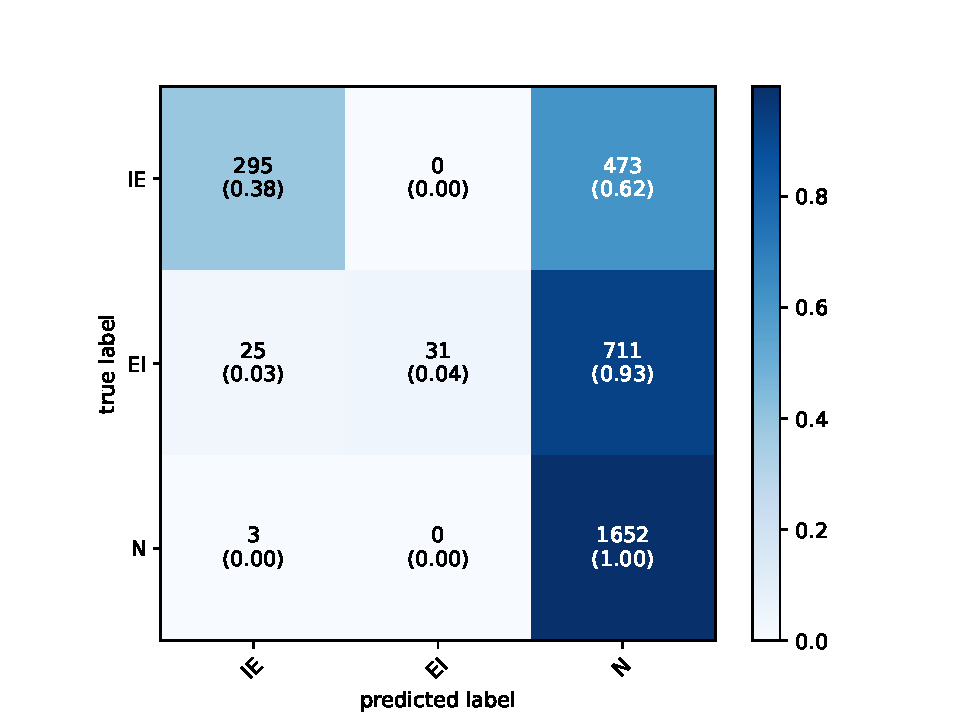
\includegraphics[width=0.6\textwidth]{figures/dna-rules-confusion-matrix}
    \end{figure}
    %
    
    \framebreak
    
    \begin{figure}
        \centering
        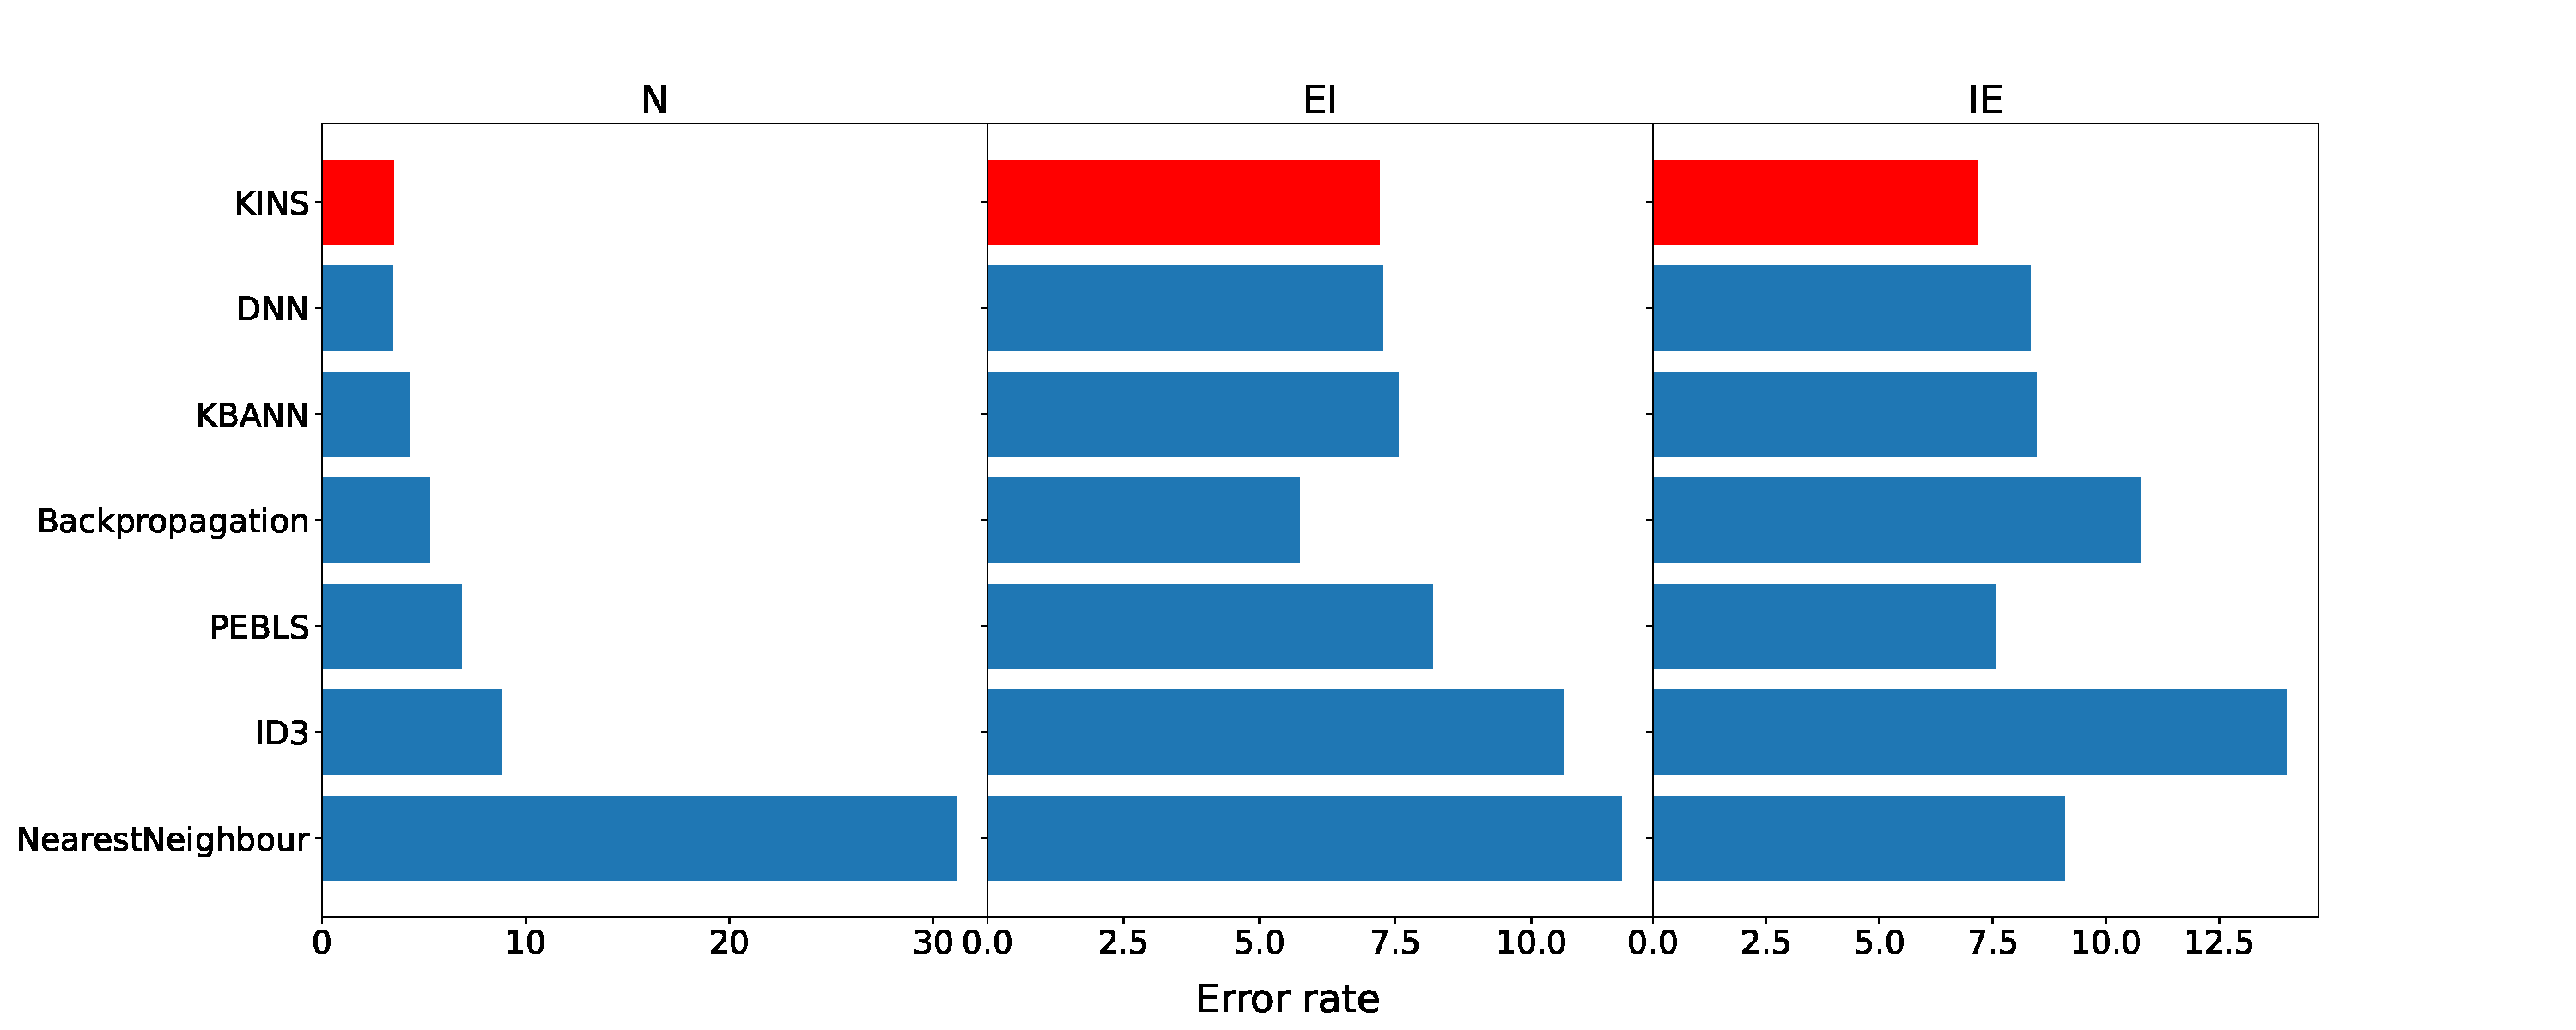
\includegraphics[width=\textwidth]{figures/kins-error-rate}
    \end{figure}
    %
    
\end{frame}
%/////////


%/////////
\begin{frame}[allowframebreaks]{\longkill}
    \begin{block}{\longkill{} (\shortkill)}
        %
        A general SKI algorithm that does not impose constrains on the sub-symbolic predictor to enrich, except being a neural network.
        %
        \begin{itemize}
            %
            \item aim $\rightarrow$ enrich;
            %
            \item predictor $\rightarrow$ neural network;
            %
            \item how $\rightarrow$ constraining;
            %
            \item logic $\rightarrow$ stratified Datalog with negation.
            %    
        \end{itemize}
    \end{block}
    
    \framebreak
    
    \begin{figure}
        \centering
        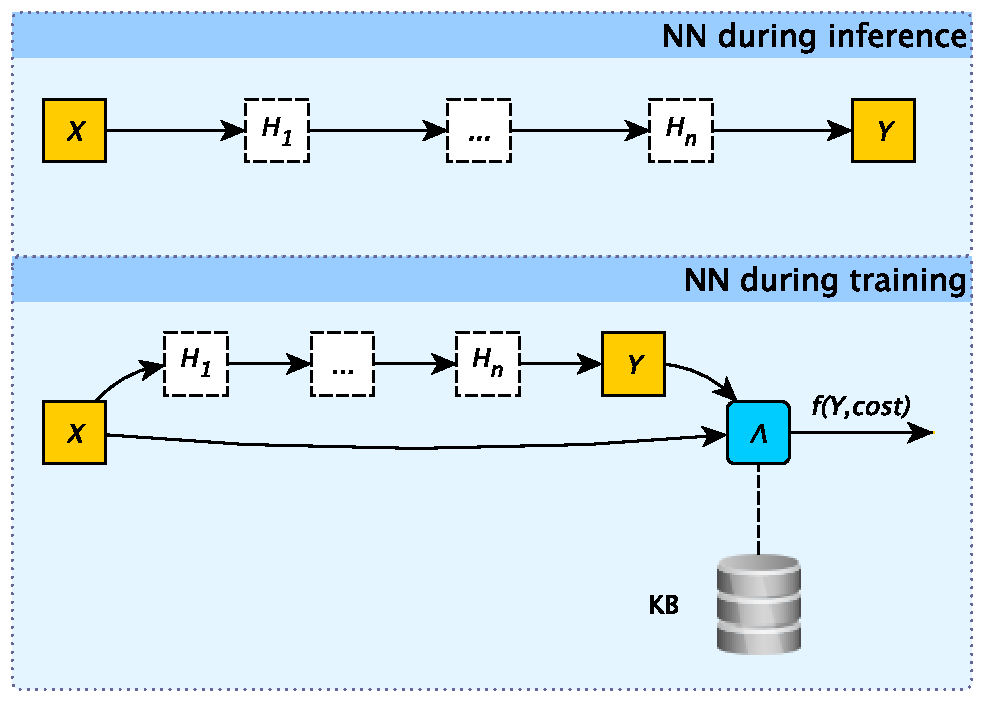
\includegraphics[width=0.8\textwidth]{figures/lambda-layer.pdf}
    \end{figure}
    
    \framebreak
    
    % !TeX spellcheck = en_GB
% !TeX root = ../ski-uai-2022.tex

\begin{table}%[!h]
    \centering
    \resizebox{\textwidth}{!}{%
        %
        %\caption{
            %Logic formul\ae's encoding into real-valued functions.
            %
            %There, $X$ is a logic variable, while $x$ is the corresponding real-valued variable, whereas is $\bar{X}$ a tuple of logic variables.
            %
            %Similarly, $\const{k}$ is a numeric constant, and $k$ is the corresponding real value, whereas $\const{k}_i$ is the constant denoting the $i^{th}$ class of a classification problem.
            %
            %Finally, $\text{expr}(\bar{X})$ is an arithmetic expression involving the variables in $\bar{X}$.
        %}
        %
        \label{tab:logic-formulae}
        %
        \begin{tabular}{l|r||cl|r}
            \textbf{Formula} & \textbf{C. interpretation} & & \textbf{Formula} & \textbf{C. interpretation}
            \\
            \hline\hline
            $\llbracket\neg \phi\rrbracket$ & $\eta(1 - \llbracket\phi\rrbracket)$ & & $\llbracket\phi \le \psi\rrbracket$  & $\eta(\llbracket\phi\rrbracket - \llbracket\psi\rrbracket)$
            \\
            $\llbracket\phi  \wedge \psi\rrbracket$ &  $\eta(max(\llbracket\phi\rrbracket, \llbracket\psi\rrbracket))$ & & $\llbracket \pred{class}(\bar{X}, \const{y}_i) \leftarrow \psi \rrbracket$ & $\llbracket \psi \rrbracket^{*}$
            \\
            $\llbracket\phi  \vee \psi\rrbracket$ & $\eta(min(\llbracket\phi\rrbracket, \llbracket\psi\rrbracket))$ & & $\llbracket \text{expr}(\bar{X}) \rrbracket$ & $\text{expr}(\llbracket\bar{X}\rrbracket)$
            \\
            $\llbracket\phi = \psi\rrbracket$ & $\eta(|\llbracket\phi\rrbracket-\llbracket\psi\rrbracket|)$ & & $\llbracket \mathtt{true} \rrbracket$ & $0$
            \\
            $\llbracket\phi \ne \psi\rrbracket$ & $\llbracket \neg ( \phi = \psi )\rrbracket$ & & $\llbracket \mathtt{false} \rrbracket$ & $1$
            \\
            $\llbracket\phi > \psi\rrbracket$  & $\eta(0.5 - \llbracket\phi\rrbracket + \llbracket\psi\rrbracket) $ & & $\llbracket X \rrbracket$ & $x$
            \\
            $\llbracket\phi \ge \psi\rrbracket$ & $\eta(\llbracket\psi\rrbracket - \llbracket\phi\rrbracket)$ & & $\llbracket \const{k} \rrbracket$ & $k$
            \\
            $\llbracket\phi < \psi\rrbracket$  &  $\eta(0.5 + \llbracket\phi\rrbracket - \llbracket\psi\rrbracket)$ & & $\llbracket \pred{p}(\bar{X}) \rrbracket^{**}$ & $\llbracket \psi_1 \vee \ldots \vee \psi_k \rrbracket$
            
        \end{tabular}
    }
    %
    \begin{center}\scriptsize
        $^{*}$ encodes the penalty for the $i^{th}$ neuron
        \\
        \smallskip
        $^{**}$ assuming predicate $p$ is defined by $k$ clauses of the form:
        \\
        $\pred{p}(\bar{X}) \leftarrow \psi_1,\ \ldots,\ \pred{p}(\bar{X}) \leftarrow \psi_k$
    \end{center}
\end{table}
    
    \framebreak
    
    \begin{block}{Cost function}
        Whenever the neural network wrongly predicts a class and violates the prior knowledge a cost proportional to the violation is added.
        %
        In this way the output of the network differs more from the expected one and this affects the back propagation step.
    \end{block}
    
    \begin{equation*}
        \centering
        \begin{aligned}
            &Y' = f(Y, \pred{cost})\\
            &f = Y\ x\ (\textbf{1} + \pred{cost})\\
            &\pred{cost}(X,Y) = \eta(\pred{p}(X) - (\textbf{1} - Y))\quad \text{(}\textbf{1} - Y\text{ because 0 means true)}\\
        \end{aligned}
    \end{equation*}
    
    \framebreak
    
    \begin{figure}
        \centering
        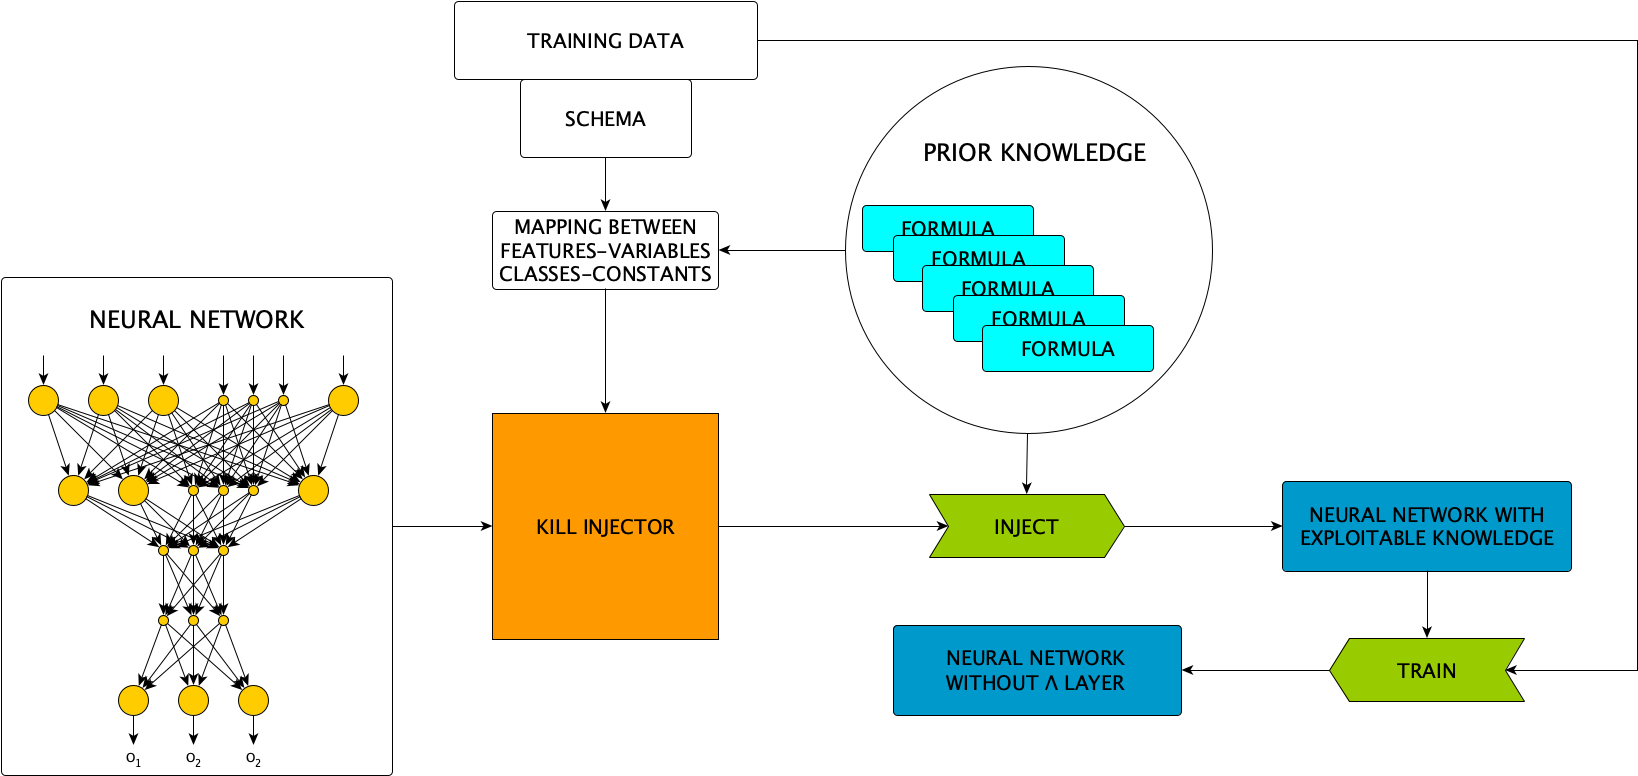
\includegraphics[width=0.9\textwidth]{figures/kill.png}
    \end{figure}
    
\end{frame}


%/////////
\begin{frame}[allowframebreaks]{Case study}
    
    \begin{block}{PHDS: Poker Hand Data Set}
        Each record represents one poker hand. 5 cards identified by 2 values: suit and rank.
        %
        Classes: 10.
        %
        Training set: 25.010. Test set: 1.000.000.
    \end{block}
    
    
\begin{table}%[!h]
    \centering
    \resizebox{0.65\textwidth}{!}{%
        \label{tab:poker-data}
        %
        \begin{tabular}{l|l|l|l|l|l|l|l|l|l|l|r}
            \textbf{id} & \textbf{S1} & \textbf{R1} & \textbf{S2} & \textbf{R2} & \textbf{S3} & \textbf{R3} & \textbf{S4} & \textbf{R4} & \textbf{S5} & \textbf{R5} & \textbf{class}\\
            \hline\hline
            1 & 1 & 10 & 1 & 11 & 1 & 13 & 1 & 12 & 1 & 1 & 9\\
            2 & 2 & 11 & 2 & 13 & 2 & 10 & 2 & 12 & 2 & 1 & 9\\
            3 & 3 & 12 & 3 & 11 & 3 & 13 & 3 & 10 & 3 & 1 & 9\\
            4 & 4 & 10 & 4 & 11 & 4 & 1 & 4 & 13 & 4 & 12 & 9\\
            5 & 4 & 1 & 4 & 13 & 4 & 12 & 4 & 11 & 4 & 10 & 9\\
            6 & 1 & 2 & 1 & 4 & 1 & 5 & 1 & 3 & 1 & 6 & 8\\
            7 & 1 & 9 & 1 & 12 & 1 & 10 & 1 & 11 & 1 & 13 & 8\\
            8 & 2 & 1 & 2 & 2 & 2 & 3 & 2 & 4 & 2 & 5 & 8\\
            9 & 3 & 5 & 3 & 6 & 3 & 9 & 3 & 7 & 3 & 8 & 8\\
            10 & 4 & 1 & 4 & 4 & 4 & 2 & 4 & 3 & 4 & 5 & 8\\
            11& 1 & 1 & 2 & 1 & 3 & 9 & 1 & 5 & 2 & 3 & 1\\
            12 & 2 & 6 & 2 & 1 & 4 & 13 & 2 & 4 & 4 & 9 & 0\\
            13 & 1 & 10 & 4 & 6 & 1 & 2 & 1 & 1 & 3 & 8 & 0\\
            14 & 2 & 13 & 2 & 1 & 4 & 4 & 1 & 5 & 2 & 11 & 0\\
            15 & 3 & 8 & 4 & 12 & 3 & 9 & 4 & 2 & 3 & 2 & 1\\
        \end{tabular}
    }
%
\end{table}
    
    \framebreak
    
    Some injected rules.
    \begin{scriptsize}
    \begin{longtable}{|p{1.5cm}|p{9cm}}
            \textbf{Class} & \textbf{Logic Formulation}
            \\\hline\hline
            Pair & $\begin{array}{l}
                \pred{class}(R_1, \ldots, S_5, \const{pair}) \leftarrow \pred{pair}(R_1, \ldots, S_5)
                \\
                \pred{pair}(R_1, \ldots, S_5) \leftarrow R_1 = R_2
                \\
                \pred{pair}(R_1, \ldots, S_5) \leftarrow R_1 = R_3
                \\
                \pred{pair}(R_1, \ldots, S_5) \leftarrow R_1 = R_4
                \\
                \pred{pair}(R_1, \ldots, S_5) \leftarrow R_1 = R_5
                \\
                \pred{pair}(R_1, \ldots, S_5) \leftarrow R_2 = R_3
                \\
                \pred{pair}(R_1, \ldots, S_5) \leftarrow R_2 = R_4
                \\
                \pred{pair}(R_1, \ldots, S_5) \leftarrow R_2 = R_5
                \\
                \pred{pair}(R_1, \ldots, S_5) \leftarrow R_3 = R_4
                \\
                \pred{pair}(R_1, \ldots, S_5) \leftarrow R_3 = R_5
                \\
                \pred{pair}(R_1, \ldots, S_5) \leftarrow R_4 = R_5
            \end{array}$
            \\\hdashline
            Two Pairs & $\begin{array}{l}
                \pred{class}(R_1, \ldots, S_5, \const{two}) \leftarrow \pred{two}(R_1, \ldots, S_5)
                \\
                \pred{two}(R_1, \ldots, S_5) \leftarrow R_1 = R_2 \wedge R_3 = R_4
                \\
                \pred{two}(R_1, \ldots, S_5) \leftarrow R_1 = R_3 \wedge R_2 = R_4
                \\
                \pred{two}(R_1, \ldots, S_5) \leftarrow R_1 = R_4 \wedge R_2 = R_3
                \\
                \pred{two}(R_1, \ldots, S_5) \leftarrow R_1 = R_2 \wedge R_3 = R_5
                \\
                \pred{two}(R_1, \ldots, S_5) \leftarrow R_1 = R_3 \wedge R_3 = R_5
                \\
                \pred{two}(R_1, \ldots, S_5) \leftarrow R_1 = R_5 \wedge R_2 = R_3
                \\
                \pred{two}(R_1, \ldots, S_5) \leftarrow R_1 = R_2 \wedge R_4 = R_5
                \\
                \pred{two}(R_1, \ldots, S_5) \leftarrow R_1 = R_4 \wedge R_2 = R_5
                \\
                \pred{two}(R_1, \ldots, S_5) \leftarrow R_1 = R_5 \wedge R_2 = R_4
                \\
                \pred{two}(R_1, \ldots, S_5) \leftarrow R_1 = R_3 \wedge R_4 = R_5
                \\
                \pred{two}(R_1, \ldots, S_5) \leftarrow R_1 = R_4 \wedge R_3 = R_5
                \\
                \pred{two}(R_1, \ldots, S_5) \leftarrow R_1 = R_5 \wedge R_3 = R_4
                \\
                \pred{two}(R_1, \ldots, S_5) \leftarrow R_2 = R_3 \wedge R_4 = R_5
                \\
                \pred{two}(R_1, \ldots, S_5) \leftarrow R_2 = R_4 \wedge R_3 = R_5
                \\
                \pred{two}(R_1, \ldots, S_5) \leftarrow R_2 = R_5 \wedge R_3 = R_4
            \end{array}$
            \\\hdashline
            Three of a Kind & $\begin{array}{l}

                \pred{class}(R_1, \ldots, S_5, \const{three}) \leftarrow \pred{three}(R_1, \ldots, S_5)
                \\
                \pred{three}(R_1, \ldots, S_5) \leftarrow R_1 = R_2 \wedge R_1 = R_3
                \\
                \pred{three}(R_1, \ldots, S_5) \leftarrow R_1 = R_2 \wedge R_1 = R_4
                \\
                \pred{three}(R_1, \ldots, S_5) \leftarrow R_1 = R_2 \wedge R_1 = R_5
                \\
                \pred{three}(R_1, \ldots, S_5) \leftarrow R_1 = R_3 \wedge R_1 = R_4
                \\
                \pred{three}(R_1, \ldots, S_5) \leftarrow R_1 = R_3 \wedge R_1 = R_5
                \\
                \pred{three}(R_1, \ldots, S_5) \leftarrow R_1 = R_4 \wedge R_1 = R_5
                \\
                \pred{three}(R_1, \ldots, S_5) \leftarrow R_2 = R_3 \wedge R_2 = R_4
                \\
                \pred{three}(R_1, \ldots, S_5) \leftarrow R_2 = R_3 \wedge R_2 = R_5
                \\
                \pred{three}(R_1, \ldots, S_5) \leftarrow R_2 = R_4 \wedge R_2 = R_5
                \\
                \pred{three}(R_1, \ldots, S_5) \leftarrow R_3 = R_4 \wedge R_3 = R_5
                
            \end{array}$
            \\\hdashline
            Flush & $\begin{array}{l}

                \pred{class}(R_1, \ldots, S_5, \const{flush}) \leftarrow \pred{flush}(R_1, \ldots, S_5)
                \\
                \pred{flush}(R_1, \ldots, S_5) \leftarrow S_1 = S_2 \wedge S_1 = S_3 \wedge S_1 = S_4 \wedge S_1 = S_5

            \end{array}$
            \\\hdashline
            Four of a Kind & $\begin{array}{l}

                \pred{class}(R_1, \ldots, S_5, \const{four}) \leftarrow \pred{four}(R_1, \ldots, S_5)
                \\
                \pred{four}(R_1, \ldots, S_5) \leftarrow R_1 = R_2 \wedge R_1 = R_3 \wedge R_1 = R_4
                \\
                \pred{four}(R_1, \ldots, S_5) \leftarrow R_1 = R_2 \wedge R_1 = R_3 \wedge R_1= R_5
                \\
                \pred{four}(R_1, \ldots, S_5) \leftarrow R_1 = R_2 \wedge R_1 = R_4 \wedge R_1 = R_5
                \\
                \pred{four}(R_1, \ldots, S_5) \leftarrow R_1 = R_3 \wedge R_1 = R_4 \wedge R_1 = R_5
                \\
                \pred{four}(R_1, \ldots, S_5) \leftarrow R_2 = R_3 \wedge R_2 = R_4 \wedge R_2 = R_5

            \end{array}$
        \end{longtable}
\end{scriptsize}
    
    \framebreak
    
    \begin{block}{Setup}
        \begin{itemize}
            \item neural network: 3-layers fully connected (128, 128, 10 neurons per layer respectively) with rectified linear unit (ReLU) as activation function, except for the last layer (softmax);
            %
            \item knowledge: see previous slides;
            %
            \item categorical cross-entropy as loss function
            %
            \item training: Adams as optimiser for 100 epochs (with early stop conditions);
            %
            \item experiment repeated 30 times to have a statistic significant population.
        \end{itemize}
    \end{block}
    %
    
    \framebreak
    
    \begin{table}[!h]
    \centering
    \begin{adjustbox}{width=\linewidth,center}
         \begin{tabular}{l|rr||l|rr}
             \textbf{Metric} & \textbf{Classic} & \textbf{\shortkill} & \textbf{Metric} & \textbf{Classic} & \textbf{\shortkill}
             \\
             \hline\hline
             \textbf{Accuracy} & 0.962 & 0.978 & \textbf{Acc. Straight} & 0.415 & 0.509
             \\
             \textbf{Macro-F1} & 0.512 & 0.538 & \textbf{Acc. Flush} & 0.002 & 0.002
             \\
             \textbf{Weighted-F1} & 0.96 & 0.977 & \textbf{Acc. Full} & 0.628 & 0.69
             \\
             \textbf{Acc. Nothing} & 0.977 & 0.989 & \textbf{Acc. Four} & 0.186 & 0.19
             \\
             \textbf{Acc. Pair} & 0.968 & 0.985 & \textbf{Acc. Straight F.} & 0.003 & 0
             \\
             \textbf{Acc. Two Pairs} & 0.867 & 0.914 & \textbf{Acc. Royal F.} & 0 & 0
             \\
             \textbf{Acc. Three} & 0.913 & 0.922 & & &
        \end{tabular}
    \end{adjustbox}
    \label{tab:test-stats}
\end{table}
    
    \framebreak
    
    \begin{figure}
        \centering
        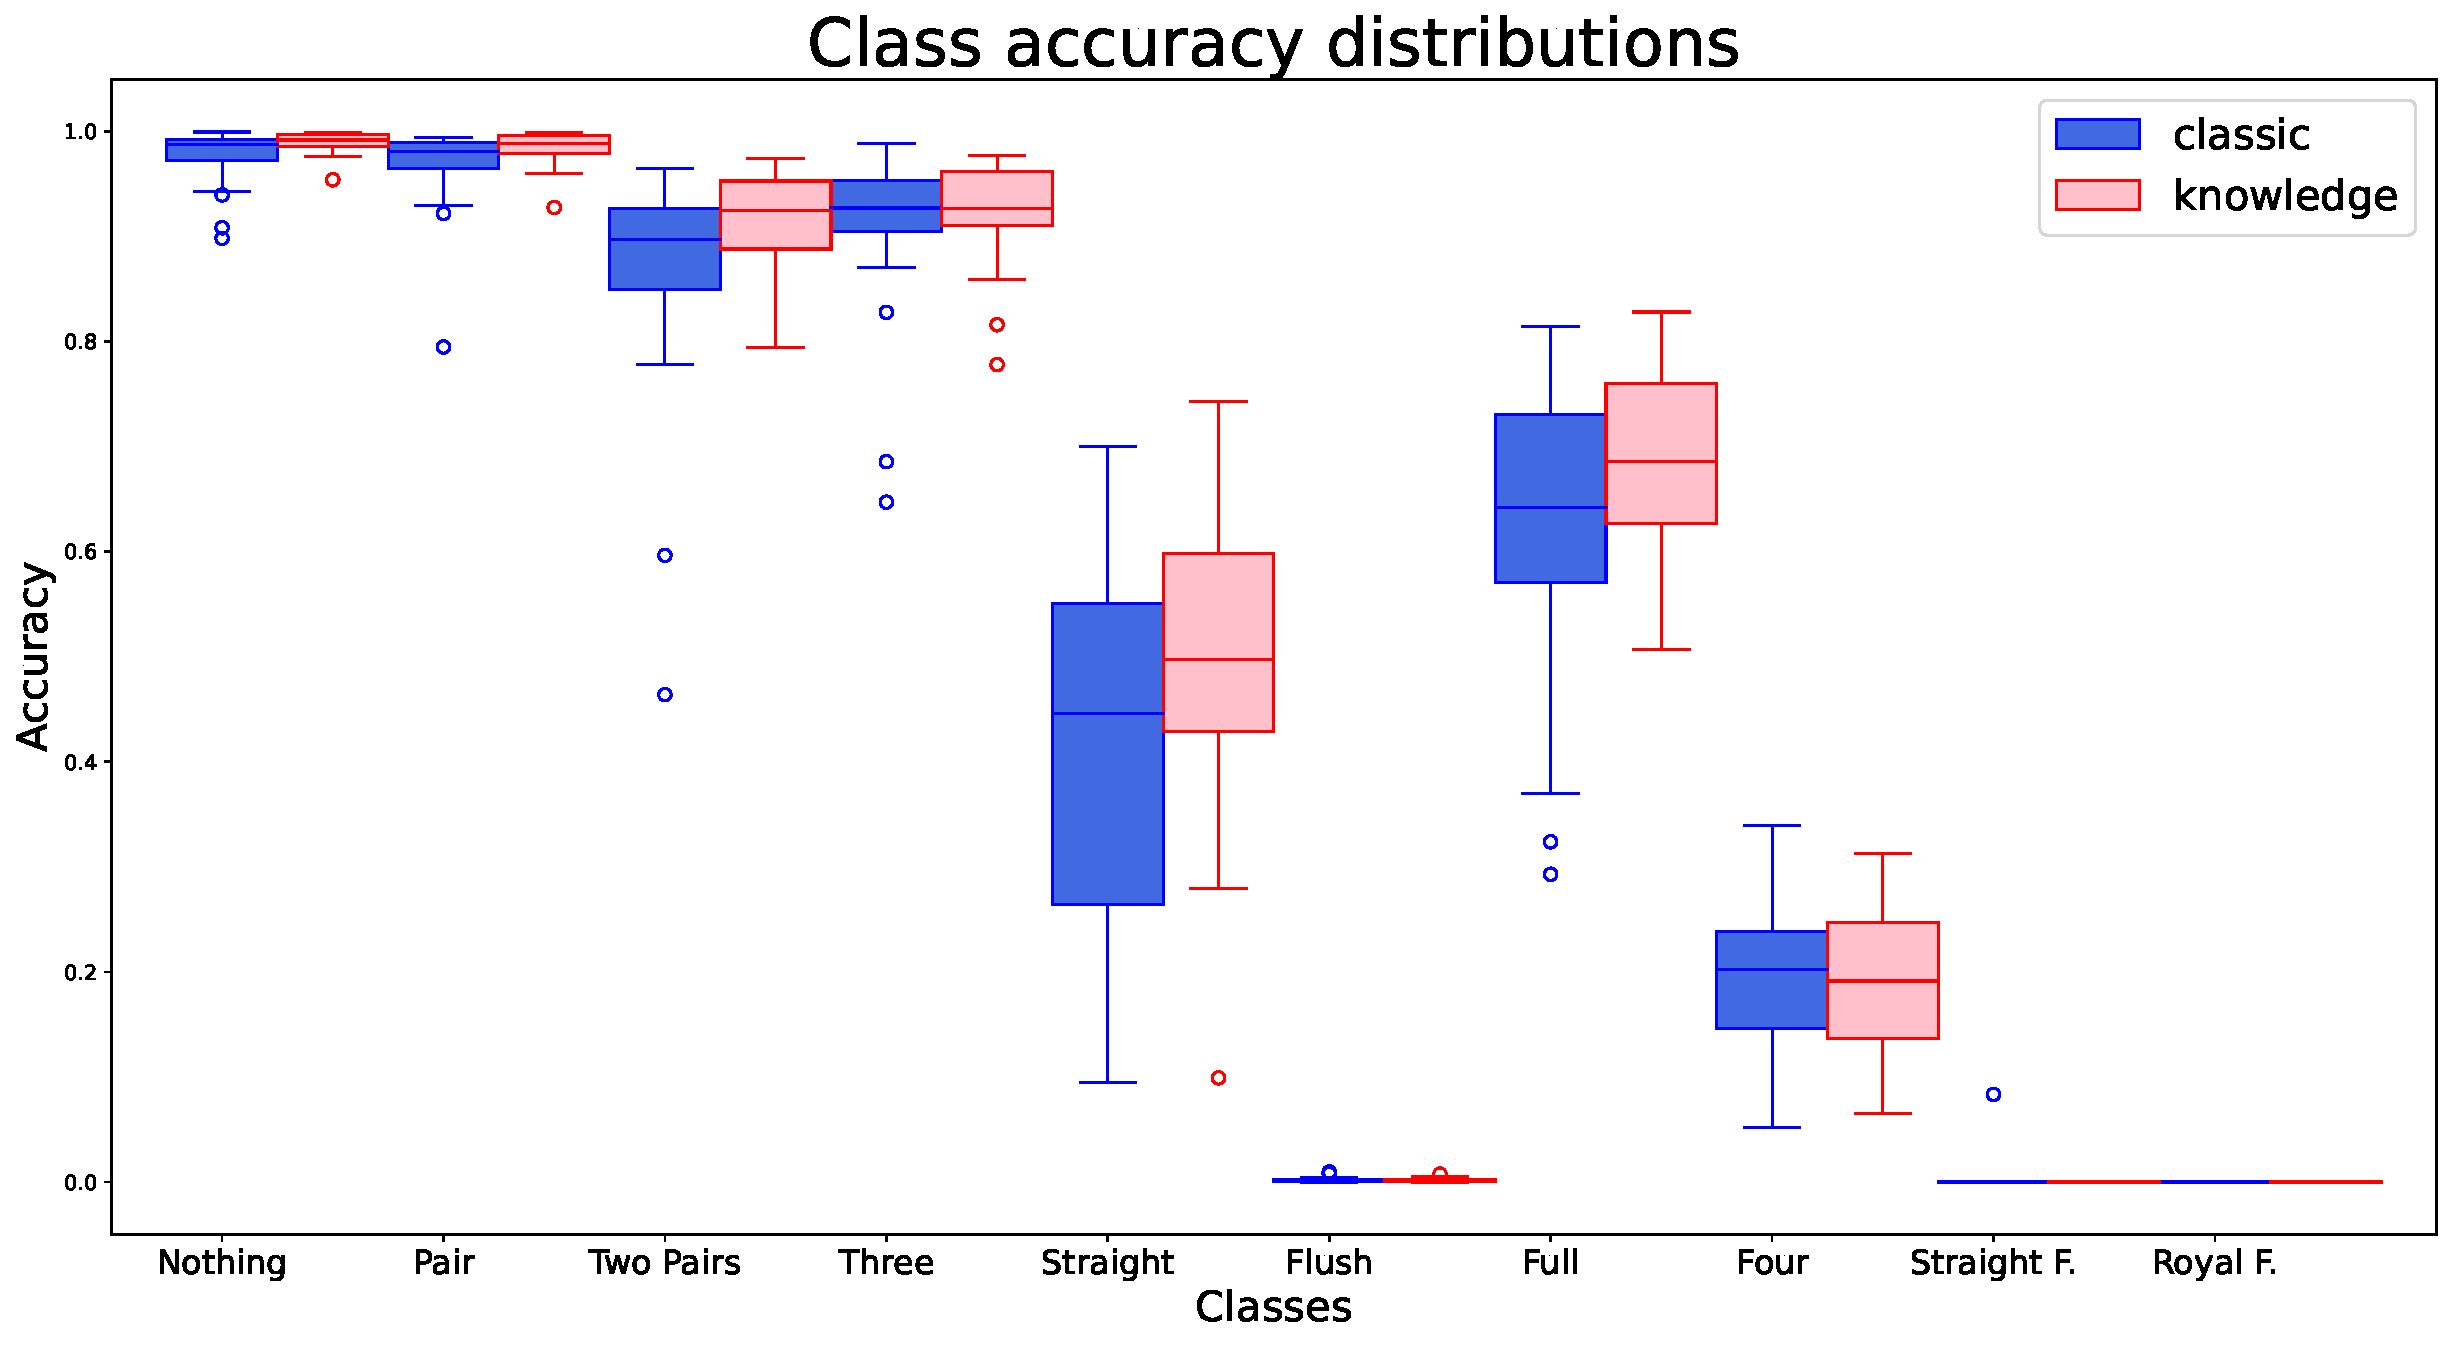
\includegraphics[width=.8\linewidth]{figures/class-accuracy-distributions.pdf}
    \end{figure}
    
\end{frame}


%===============================================================================
\section{Open literature research lines}
%===============================================================================


%/////////
\begin{frame}[c]{SKE \& SKI}
    %
    \begin{figure}
        \centering
        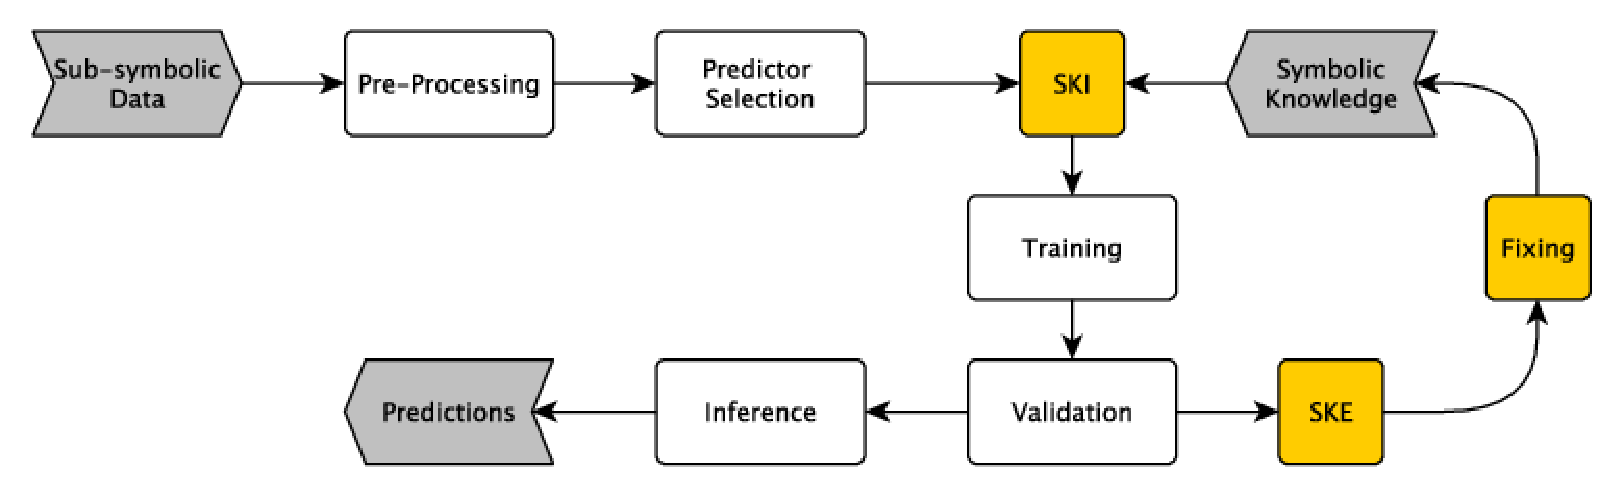
\includegraphics[width=\textwidth]{figures/ske-ski-workflow}
    \end{figure}
\end{frame}
%/////////


%/////////
\begin{frame}[c]{Multi-Agent Systems}
    %
    \begin{itemize}
        \item agent to agent explanation \ccite{explanation-aixia2020dp}\\
        %
        $\rightarrow$ SKE + SKI + explanation;
        %
        \item logic as lingua franca for communication between heterogeneous entities;
        %
        \item knowledge sharing and knowledge exploitation among agents;
        %
        \item symbolic techniques integrated with sub-symbolic ones\\
        %
        $\rightarrow$ representing and manipulating cognitive
        processes and their results.
    \end{itemize}
\end{frame}
%/////////

%===============================================================================
\section*{}
%===============================================================================

%/////////
\frame{\titlepage}
%/////////

%===============================================================================
\section*{\refname}
%===============================================================================

%%%%
\setbeamertemplate{page number in head/foot}{}
%/////////
%\begin{frame}[c,noframenumbering]{\refname}
\begin{frame}[t,allowframebreaks,noframenumbering]{\refname}
    %	\tiny
    \scriptsize
    %	\footnotesize
    \bibliographystyle{apalike-AMS}
    \bibliography{ske-ski-talk-2022}
\end{frame}
%/////////

%%%%%%%%%%%%%%%%%%%%%%%%%%%%%%%%%%%%%%%%%%%%%%%%%%%%%%%%%%%%%%%%%%%%%%%%%%%%%%%%
\end{document}
%%%%%%%%%%%%%%%%%%%%%%%%%%%%%%%%%%%%%%%%%%%%%%%%%%%%%%%%%%%%%%%%%%%%%%%%%%%%%%%%
